
\chapter{Elementary data structures}

This chapter will describe in detail the most common data structures and their implementations in KamilaLisp. Many data structures in KamilaLisp are defined in terms of each other - for instance, all the functions that generally operate on sets can also be used on lists, since sets constitute a special case of lists. This chapter will also describe elementary array programming in KamilaLisp, which is usually the preferred by many programmers way to solve complex problems quickly.

\section{Basic list operations}

Lists are one of the most important data structures used in functional programming. Every major programming language provides means of finite sequence storage and KamilaLisp is no different. A special emphasis is put on list and array processing, the basic building block of dataflow programming.

As mentioned before, every list besides the empty list contains a \textit{head} (the first element, \verb|car|) and a \textit{tail} (the last element, \verb|cdr|). The tail of a list is always another list, even if it is empty. The empty list literal is introduced in the code as \verb|'nil| or \verb|'()|. 

Using \verb|car| and \verb|cdr| it is possible to define a basic, non-tail recursive function that yields the length of a list:

\begin{Verbatim}
    --> defun length l (if (same l 'nil) 0 (+ 1 (length (cdr l))))
    (λ l . (if (same l 'nil) 0 (+ 1 (length (cdr l)))))
\end{Verbatim}

A generalised version of this function that handles scalar values, variadic application and strings is available as \verb|tally|\footnote{\textit{tally} - to count or calculate something}:

\begin{Verbatim}
    --> tally '(1 2 3) '(4 5)
    (3 2)
    --> tally '(1 2 3 4 5)
    5
    --> tally "abcde"
    5
    --> tally 5
    1
    --> tally
    0
\end{Verbatim}

Individual elements may be prepended to a list using the \verb|cons| function:

\begin{Verbatim}
    --> cons 6 'nil
    (6)
    --> cons 5 (cons 6 'nil)
    (5 6)
    --> cons 1 '(2 3)
    (1 2 3)
\end{Verbatim}

Hence, one could define a countdown function as follows:

\begin{Verbatim}
    --> defun countdown x (if x (cons x (countdown (- x 1))) '(0))
    (λ x . (if x (cons x (countdown (- x 1))) '(0)))
    --> countdown 5
    (5 4 3 2 1 0)
\end{Verbatim}

Once again, a general result of this function is available in KamilaLisp as the \verb|range| function:

\begin{Verbatim}
    --> range 5
    (0 1 2 3 4)
    --> range 5 10
    (5 6 7 8 9)
    --> range 10 5
    (10 9 8 7 6)
    --> range 5 -5
    (5 4 3 2 1 0 -1 -2 -3 -4)
\end{Verbatim}

List concatenation in KamilaLisp is accomplished using the \verb|append| function. The \verb|append| function is of course variadic and accepts an empty parameter list:

\begin{Verbatim}
    --> append '(1 2 3) '(4 5)
    (1 2 3 4 5)
    --> append '(1 2 3) '(4 5) '(6 7)
    (1 2 3 4 5 6 7)
    --> append
    'nil
    --> append 'nil 'nil
    'nil
    --> append "Tomato" "sauce"
    Tomatosauce
\end{Verbatim}

Prefixes and suffixes of lists may be extracted using the \verb|take| and \verb|drop| functions as follows:

\begin{Verbatim}
    --> take 3 '(1 2 3 4 5)
    (1 2 3)
    --> drop 3 '(1 2 3 4 5)
    (4 5)
    --> take 3 '(1 2 3)
    (1 2 3)
    --> drop 3 '(1 2 3)
    --> take 3 'nil
    [[]
     []
     []]
    --> drop 3 'nil
    --> take 5 '(1 2 3)
    (1 2 3 0 0)
\end{Verbatim}

The \verb|take| and \verb|drop| functions also accept negative argument, which changes the direction of the operation:

\begin{Verbatim}
    --> take -3 "KamilaLisp is Fun"
    Fun
\end{Verbatim}

More generally, \textit{all} prefixes and suffixes of a list are extracted using the \verb|prefixes| and \verb|suffixes| functions:

\begin{Verbatim}
    --> prefixes '(1 2 3 4 5)
    ((1) (1 2) (1 2 3) (1 2 3 4) (1 2 3 4 5))
    --> suffixes '(1 2 3 4 5)
    ((1 2 3 4 5) (2 3 4 5) (3 4 5) (4 5) (5))
    --> suffixes "Lisp"
    ("Lisp" "isp" "sp" "p")
\end{Verbatim}

Going back to the \verb|take| function, it is easy to notice that when the list is shorter than expected, the resultant list is simply padded with zeroes. This may not be the desired behaviour, thus a variant of \verb|take| called \verb|cycle| is provided. The \verb|cycle| function takes a list and a number and returns a list of the same length as the number, where the elements are taken from the list in a cyclic manner:

\begin{Verbatim}
    --> cycle 5 '(1 2 3)
    (1 2 3 1 2)
    --> cycle 3 '(1 2 3)
    (1 2 3)
    --> cycle 2 '(1 2 3)
    (1 2)
    --> cycle 1 '(1 2 3)
    (1)
    --> cycle 0 '(1 2 3)
    --> cycle -1 '(1 2 3)
    RuntimeException thrown in thread 1dbd16a6:
            cycle: negative length
        at entity cycle  1:1
        at cycle primitive function
    --> cycle 'nil 5
    --> cycle "abc" 5
    abcab
\end{Verbatim}

The \verb|replicate| function ubiquitously used in APL and Haskell is also available in KamilaLisp, except its domain is extended to scalar values:

\begin{Verbatim}
    --> replicate 3 5
    (5 5 5)
    --> replicate 5 '(1 2 3)
    (1 2 3 1 2 3 1 2 3 1 2 3 1 2 3)
    --> replicate 5 "Kamila"
    KamilaKamilaKamilaKamilaKamila
    --> replicate 0 5
    --> replicate 5 'nil
    --> replicate '(1 2 3) '(4 5 6)
    (4 5 5 6 6 6)
\end{Verbatim}

KamilaLisp also provides a few functions for altering the \textit{order} of elements in a list. The \verb|reverse| function reverses the order of elements in a list:

\begin{Verbatim}
    --> reverse '(1 2 3 4 5)
    (5 4 3 2 1)
    --> reverse "KamilaLisp"
    psiLalimaK
\end{Verbatim}

The \verb|rotate| function, as the name suggests, takes a list and a number and returns a list where the elements are rotated by the number of slots:

\begin{Verbatim}
    --> rotate 2 '(1 2 3 4 5)
    (3 4 5 1 2)
    --> rotate -2 '(1 2 3 4 5)
    (4 5 1 2 3)
    --> rotate -4 "KamilaLisp"
    LispKamila
    --> rotate 1 'nil
    --> rotate 0 'nil
\end{Verbatim}

Finally, the \verb|list:shuffle| function will take a list and return a list with the same elements, but in a random order:

\begin{Verbatim}
    --> list:shuffle '(1 2 3 4 5)
    (2 5 3 1 4)
    --> list:shuffle "KamilaLisp"
    LpLsikmaia
\end{Verbatim}

\section{Sorting, searching and indexing}

KamilaLisp defines a special syntax for indexing into lists. The syntax is as follows:

\begin{Verbatim}
    --> def x '(1 5 2 3 4)
    (1 5 2 3 4)
    --> ?x$[0]
    1
\end{Verbatim}

This syntax is very confusing when demonstrated in isolation. First, indexing returns a value without a function call involved, so it is mandatory to tell the interpreter that the intent is to obtain the value of an object, hence the \verb|?| prefix in the REPL. It is possible to index a list using a list, as follows:

\begin{Verbatim}
    --> ?x$[1 3 4]
    (5 3 4)
\end{Verbatim}

The indexing function loops over the list it has received and returns respectively the first, third and fourth items of a list, all tied together into a single array. This is a very powerful feature, as it allows for a very concise syntax for extracting elements from a list, applying permutations and even sorting, as demonstrated later in the book. Of course, indexing can also be done using an expression:

\begin{Verbatim}
    --> ?x$[random 5]
    3
\end{Verbatim}

Another closely related functionality related to indexing is searching. The \verb|index-of| takes a value and a list and returns the index of the first occurrence of the value in the list:

\begin{Verbatim}
    --> index-of 5 '(9 8 6 5 4 7 2 3)
    3
    --> index-of 5 '(9 8 6 4 7 2 3)
    -1
\end{Verbatim}

\section{Rank}

KamilaLisp lists have \textit{rank}, which is a measure of their nesting, usually interpreted in the context of how many dimensions they could have. For example, a doubly nested list can be interpreted as a matrix:

\begin{Verbatim}
    --> ?'((1 2) (3 4))
    [[1 2]
     [3 4]]
\end{Verbatim}

Since a matrix usually has two axes, matrices (lists of lists of scalars) have rank 2. A vector is a list of scalar values, so it has rank 1. A scalar value has rank 0. The rank of an object can be computed using the \verb|rank| function:

\begin{Verbatim}
    --> rank '((1 2) (3 4))
    2
    --> rank '(1 2 3 4)
    1
    --> rank 0
    0
\end{Verbatim}

One interesting case to consider is a \textit{ragged list} - a list whose elements have different ranks. For example, the following list is a ragged list:

\begin{Verbatim}
    --> ?'((1 2) (3 4) 5)
\end{Verbatim}

The first and second elements of the list have ranks 1 (vectors; lists of scalars), while the last element has rank 0 (a scalar). The rank of a ragged list is computed as if the maximum of ranks of a list was considered and the result is negated:

\begin{Verbatim}
    --> rank '((1 2) (3 4) 5)
    -2
\end{Verbatim}

\section{Elementary higher order functions}

KamilaLisp provides a wide variety of higher order functions for manipulating lists. Many of them can be defined using recursion, however almost all of them are guaranteed to terminate, while recursion in general case does not. The use of list processing functions that constitute the core of array programming is highly encouraged over recursion, because they tend to be more concise, easier to understand and less error prone.

The most used function is a built-in operator takes a function and a list and applies the function to each element of the list, yielding a list of the results. Define a successor function and map it over a list by prepending a single colon before the function name:

\begin{Verbatim}
    --> def s $(+ 1)
    $['+, '1]
    --> :s '(1 2 3 4 5)
    (2 3 4 5 6)
\end{Verbatim}

The \verb|map| function (which is the more familiar name of this construct, predominantly called that in Haskell and OCaml) has a few nuissances that are worth mentioning. First, it is possible to apply it to a non-list argument and an empty list:

\begin{Verbatim}
    --> :s 5
    (6)
    --> :s 'nil
    -->
\end{Verbatim}

The functor returned by \verb|:| has the same arity as the function it is applied to, hence it is possible for it to act as a \verb|zipWith| operation known from e.g. Haskell:

\begin{Verbatim}
    --> :+ '(1 2 3) '(4 5 6)
    (5 7 9)
    --> :+ '(1 2 3) '(4 5 6 7)
    (5 7 9)
    --> :+ '(1 2 3 4) '(4 5 6)
    (5 7 9)
    --> :+ '(1 1 1) '(2 2 2) '(3 3 3)
    (6 6 6)
\end{Verbatim}

To present an example, the colon operator would be helpful in implementing a function to test whether its arguments are monotonically increasing or decreasing. The notation $x \le y \le z$ does not quite translate to KamilaLisp:

\begin{Verbatim}
    --> < 1 2 3
    TypeError thrown in thread 9225652:
        2 arguments expected in application.
    at entity <  1:1
    at < primitive function
\end{Verbatim}

A function called \verb|monotonic| can be defined to test whether a list of numbers is monotonically increasing or decreasing\footnote{Monotonically decreasing means that every element of a sequence is smaller than the previous element.}, based on the comparison function it takes argument:

\begin{Verbatim}
    --> defun monotonic (fn list) (same '(1) (unique (:fn list (cdr list))))
    (λ fn list . (same '(1) (unique (:fn list (cdr list)))))
    --> monotonic < '(1 2 3)
    1
    --> monotonic < '(1 4 3)
    0
\end{Verbatim}

This particular example uses slightly inefficient logic (takes all unique elements of the mapping and checks if the resultant list is a singleton list\footnote{A list containing only one element} of \verb|1|), while a more efficient implementation would use a higher order function to test whether all the elements of the resultant list are \verb|1|, however this topic will be covered later on in the book.

Coming back to \verb|map|, it is possible to specify \textit{invariant arguments} to the function - the invariant arguments are constant arguments that are always supplied to the function being mapped, while other arguments over which \verb|map| can iterate are changing:

\begin{Verbatim}
    --> :+ 5 '(5) '(1 2 3 4 5)
    (11 12 13 14 15)
\end{Verbatim}

An important observation to be made is that it is possible to apply a function to a list of lists by stacking the comma operator multiple times also utilising the invariant arguments to write a function that forms tuples from the elements in a two-dimensional matrix:

\begin{Verbatim}
    --> def mat '((4 3) (3 4))
    [[4 3]
     [3 4]]
    --> ::cons 5 mat
    (((5 4) (5 3)) ((5 3) (5 4)))
\end{Verbatim}

The colon operator may not be general enough to be suitable for all uses. For example, it may be desirable to create a \textit{pervasive function} - a function which automatically applies itself to all the scalar values in a list. The built-in functions such as \verb|+|, \verb|-| or \verb|ln| are pervasive by default, but for example the \verb|reverse| function is not:

\begin{Verbatim}
    --> reverse '(("hi" "hello") ("kamila" "lisp"))
    (("kamila" "lisp") ("hi" "hello"))
\end{Verbatim}

Since strings are generally considered scalar values by KamilaLisp (however, this is not the case in other array programming languages such as APL), applying it \textit{on depth zero} yields the following results:

\begin{Verbatim}
    --> reverse%[0] '(("KamilaLisp" "is") "fun!")
    (("psiLalimaK" "si") "!nuf")
\end{Verbatim}

The function \verb|reverse| was ran on every object of rank zero of the list. If it is desirable reverse vectors (lists of scalars), the \verb|reverse| function should be applied \textit{on depth one}:

\begin{Verbatim}
    --> reverse%[1] '((1 2) 3 4)
    ((2 1) 3 4)
\end{Verbatim}

To give another example, to reverse the rows of a list of matrices, the function should be applied \textit{on depth two}:

\begin{Verbatim}
    --> reverse%[2] '(((1 2) (3 4)) ((5 6) (7 8)))
    (((3 4) (1 2)) ((7 8) (5 6)))
\end{Verbatim}

Of course, since the depth operator is a \textit{generalisation} of the colon operator (mapping), it is possible to use it to map a function over a list of lists. In this case, the depth specifier must be negative:

\begin{Verbatim}
    --> writeln%[-1] '("Hello" "world!")
\end{Verbatim}

The smaller negative number, the more times the map function is applied:

\begin{Verbatim}
    --> cons%[-2] mat 5
    (((4 5) (3 5)) ((3 5) (4 5)))
    --> ::cons mat 5
    (((4 5) (3 5)) ((3 5) (4 5)))
\end{Verbatim}

An important thing to note is that the depth operator subtly differs from the colon operator in the variadic case. The colon operator will determine the shape of the result ad-hoc, regardless of argument order:

\begin{Verbatim}
    --> ::cons mat 5
    (((4 5) (3 5)) ((3 5) (4 5)))
    --> ::cons 5 mat
    (((5 4) (5 3)) ((5 3) (5 4)))
\end{Verbatim}

The depth operator, however, will always infer the shape from its first argument, potentially leading to unexpected results:

\begin{Verbatim}
    --> cons%[-2] mat 5
    (((4 5) (3 5)) ((3 5) (4 5)))
    --> cons%[-2] 5 mat
    [[5 4]]
\end{Verbatim}

This behaviour significantly differs from the behaviour of the depth operator in other languages, such as APL\footnote{https://aplwiki.com/wiki/Depth\_(operator)}, where the depth operator is restricted to only two arguments, making it feasible to try dynamically determining the shape of the result. In KamilaLisp the shape is inferred from the first argument, since the operator's complexity would grow by a large magnitude as a result of it being a generalisation to an arbitrary amount of arguments. Additionally, the complex inferring rule in APL-like languages is not very useful in practice and leads to some design shortcomings.

To explore this topic further, it is necessary to demonstrate that the KamilaLisp depth operator accepts multiple depth values. For example, the following program will apply the function to objects of rank one extracted from the first array, and the objects obtained by descending once into the second array:

\begin{Verbatim}
    --> defun f (x y) (str:format "{?x}, {?y}")
    (λ x y . (str:format "{?x}, {?y}"))
    --> f%[1 -1] '((1 2) (3 4)) '(6 5 (4 3) 2 1)
    ("(1 2), 6" "(3 4), 5")
\end{Verbatim}

Notice that the depth operator makes an attempt to salvage the situation arising due to the fact that the lists are of different sizes by trimming the longer list to the size of the shorter one (which is not done by APL). To make a more fair comparison with APL, consider the following program instead:

\begin{Verbatim}
    --> f%[-2 0] '((1 2) 3) '((1 2) 3)
    (("1, 1" "2, 2") "3, 3")
\end{Verbatim}

Since the depth operator simply extracts the objects of the specified rank from the arguments, it does not pay attention to the shape of other arguments, so scalars for the second argument to f can be extracted also in this case:

\begin{Verbatim}
    --> f%[-2 0] '((1 2) 3) '(1 2 3)
    (("1, 1" "2, 2") "3, 3")
\end{Verbatim}

Since APL determines the shape in a more "clever" (also way slower and more convoluted) way, this behaviour can not be achieved:

\begin{Verbatim}
        ((1 2) 3) ({⍺⍵} ⍥ ¯2 0) (1 2) 3
┌─────────┬───┐
│┌───┬───┐│3 3│
││1 1│2 2││   │
│└───┴───┘│   │
└─────────┴───┘
        ((1 2) 3) ({⍺⍵} ⍥ ¯2 0) 1 2 3
LENGTH ERROR
        ((1 2)3)({⍺ ⍵} ⍥ ¯2 0)1 2 3
                ∧
\end{Verbatim}

Finally, the depths list can be defined as a result of an expression:

\begin{Verbatim}
    --> f%[[tie + -] 1] '((1 2) (3 4)) '(6 5 (4 3) 2 1)
    ("(1 2), 6" "(3 4), 5")
\end{Verbatim}

A function similar to list mapping is \verb|filter|. It takes a predicate and a list and returns a list of elements for which the predicate returned a truthy value.

\begin{Verbatim}
    --> filter (lambda x (> x 3)) '(1 2 3 4 5)
    (4 5)
\end{Verbatim}

The relation between \verb|filter| and \verb|map| (the colon operator) can be observed by re-implementing one in terms of the other in the following way:

\begin{Verbatim}
    --> defun my-filter (pred lst) (replicate (= 1 (:pred lst)) lst)
    (λ pred lst . (replicate (= 1 (:pred lst)) lst))
    --> my-filter (lambda x (> x 3)) '(1 2 3 4 5)
    (4 5)
\end{Verbatim}

\verb|filter| allows for an elegant yet inefficient implementation\footnote{Compared to the prime number-related primitive functions already supplied by KamilaLisp} of a prime sieve. The sieve of Eratosthenes is an algorithm for finding all prime numbers up to a given limit. It works by iteratively marking the multiples of each prime number as composite. To implement this in KamilaLisp, it is needed to use recursion and two lists of numbers: one for the primes that have been already found, and one for the numbers that have not been classified yet.

Firstly, define the iteration step function that takes the prime and unclassified lists in a pair, adds the first element from the unclassified list to the prime list and removes all its multiples from the unclassified list:

\begin{Verbatim}
    --> defun step data (let-seq
        (def primes (car data))
        (def cands (car@cdr data))
        (case (same cands 'nil) (tie primes 'nil))
        (def current (car cands))
        (tie (cons current primes) (filter $(mod _ current) (cdr cands))))
\end{Verbatim}

This example of \verb|let-seq| used the construct \verb|case|, which is a special form of \verb|if| that may be used only in \verb|let-seq|. If the condition that directly follows \verb|case| is true, then the further execution of the \verb|let-seq|'s body is stopped and the value of the expression that follows the condition is returned. This is especially useful for terminating the computation when a special case is encountered. Using \verb|while|, the iteration step function can be applied a finite amount of times to the initial pair of lists:

\begin{Verbatim}
    --> while (tie 'nil (range 2 50)) 1 step
    ((2) (3 5 7 9 11 13 15 17 19 21 23 25 27 29 31 33 35 37 39 41 43 45 47 49))
    --> while (tie 'nil (range 2 50)) 5 step
    ((11 7 5 3 2) (13 17 19 23 29 31 37 41 43 47))
    --> while (tie 'nil (range 2 50)) 10 step
    ((29 23 19 17 13 11 7 5 3 2) (31 37 41 43 47))
    --> while (tie 'nil (range 2 50)) 15 step
    ((47 43 41 37 31 29 23 19 17 13 11 7 5 3 2) nil)
    --> while (tie 'nil (range 2 50)) 20 step
    ((47 43 41 37 31 29 23 19 17 13 11 7 5 3 2) nil)
\end{Verbatim}

Since the step function \textit{converges} to a value (eventually yields a value $t$ such that $f(t) = t$), the \verb|converge| function can be used to implement most of the sieve's logic now:

\begin{Verbatim}
    --> converge step (tie 'nil (range 2 100))
    ((97 89 83 79 73 71 67 61 59 53 47 43 41 37 31 29 23 19 17 13 11 7 5 3 2) nil)
\end{Verbatim}

To provide a final result, it is necessary to extract and reverse the prime list from the pair and wrap the invocation in a function:

\begin{Verbatim}
    --> defun sieve (n) (reverse@car@converge step (tie 'nil (range 2 n)))
    (λ n . (reverse@car@converge step (tie 'nil (range 2 n))))
    --> sieve 20
    (2 3 5 7 11 13 17 19)
\end{Verbatim}

Ultimately, the function can be rewritten as follows to make it more concise and self-contained:

\begin{Verbatim}
defun sieve (n) (reverse@car@converge (
        lambda x (let-seq
            (def primes (car x))
            (def cands (car@cdr x))
            (case (same cands 'nil) (tie primes 'nil))
            (def current (car cands))
            (tie (cons current primes) (filter $(mod _ current) (cdr cands))))
    ) (tie 'nil (range 2 n)))
\end{Verbatim}

\section{Folding and scanning}

\textit{Folds} and \textit{scans} are higher-order functions that analyze a recursive data structure (usually a tree or list, however this section will focus only on folding lists) and through use of a given aggregation functor, combine the results of recursively processing its constituent parts, building up a return value. The difference between folds and scans is that the former return only the final result, while the latter return a list of intermediate results.

To demonstrate the simplest example of a fold, the sum of a list could be computed by folding it with the \verb|+| function. Of course, the order of operation in this particular case does not matter since addition is commutative, however it is common to distinguish \textit{left-associative folds} and \textit{right-associative folds}. Imagine folding a list as inserting a dyadic function between its elements:

\begin{Verbatim}
    fold - (1 2 3 4 5) = 1 - 2 - 3 - 4 - 5
\end{Verbatim}

The sum can be parenthesised in two ways: as $(((1 - 2) - 3) - 4) - 5$ or $1 - (2 - (3 - (4 - 5)))$, thus former is a left-associative fold, while the latter is a right-associative fold.

Additionally, a question arises how should folds handle empty and singleton lists. Folds, in general case, return the identity element of the aggregation functor when the list is empty. When presented with a singleton list, the fold applies the function to the identity element and the only element of the list. Obviously, it is not possible to just query the identity element of the aggregating function, which is why the identity element of it is usually passed as an argument to fold. Sometimes it is desirable to fold a list with a function that does not have an identity element, in which case folding a list with a single element returns it and folding an empty list results in an error.

Of course, all of these variants of folding have their own names in KamilaLisp:

\begin{itemize}
    \item \verb|foldl| is a left-associative fold that takes an identity element and preprends it to the input list.
    \item \verb|foldr| is a right-associative fold that takes an identity element and preprends it to the input list.
    \item \verb|foldl1| is a left-associative fold that does not take an identity element and errors on empty lists.
    \item \verb|foldr1| is a right-associative fold that does not take an identity element and errors on empty lists.
\end{itemize}

A sum from $1$ to $n$ can be naively computed using folds as follows:

\begin{Verbatim}
    --> foldl + 0 (range 1 100)
    5050
\end{Verbatim}

The direction of the fold does not matter here. However, if presented with a non-associative functor, the direction of the fold matters. Consider the following example:

\begin{Verbatim}
    --> foldl - 0 (range 1 100)
    -4950
    --> foldr - 0 (range 1 100)
    50
\end{Verbatim}

The first example essentially computes $((0 - 1) - 2) - \dots$, while the second example computes $0 - (1 - (2 - \dots))$.

The aggregating function is always a dyadic function. Depending on the direction of the fold, its arguments may be reversed. For example, in left-associative folds, the first argument is the accumulator and the second argument is the current element of the list. In right-associative folds, the first argument is the current element of the list and the second argument is the accumulator.

Folds make it possible to implement many familiar functions in a more elegant manner. Consider the arithmetic mean example introduced in the first chapter of the book:

\begin{Verbatim}
    --> defun sum (l) (if (same l '()) 0 (+ (car l) (sum (cdr l))))
    (λ l . (if (same l '()) 0 (+ (car l) (sum (cdr l)))))
    --> def mean [/ sum tally]
    [/ sum tally]
\end{Verbatim}

The \verb|mean| function can be rewritten as follows\footnote{In a very similar way to APL - compare \verb|[/ $(foldl1 +) tally]| and \verb|+/÷≢|.}:

\begin{Verbatim}
    --> def mean [/ $(foldl1 +) tally]
    [/ foldl + 0 tally]
\end{Verbatim}

Folds, in a way, transcend the concept of tail recursion. A tail-recursive \verb|foldl| function can be implemented in the following way:

\begin{Verbatim}
    --> defun my-foldl (f z l) (if (same l '()) z (&0 f (f z (car l)) (cdr l)))
    (λ f z l . (if (same l 'nil) z (&0 f (f z (car l)) (cdr l))))
    --> my-foldl - 0 (range 1 100)
    -4950
\end{Verbatim}

It is also possible to define many concept using folds, such as \verb|map| or \verb|filter|:

\begin{Verbatim}
    --> defun my-map (f l) (foldr (lambda (x y) (cons (f x) y)) 'nil l)
    (λ f l . (foldr (lambda (x y) (cons (f x) y)) 'nil l))
    --> my-map $(+ 1) (range 1 10)
    (2 3 4 5 6 7 8 9 10)
    --> defun my-filter (f l) (foldr (lambda (x y) (if (f x) (cons x y) y)) 'nil l)
    (λ f l . (foldr (lambda (x y) (if (f x) (cons x y) y)) 'nil l))
    --> my-filter $(> 5) (range 1 10)
    (1 2 3 4)
\end{Verbatim}

Perhaps more surprisingly, it is also possible to join two lists using \verb|foldr|:

\begin{Verbatim}
    --> defun my-append (l1 l2) (foldr cons l2 l1)
    (λ l1 l2 . (foldr cons l2 l1))
    --> my-append (range 1 5) (range 6 10)
    (1 2 3 4 5 6 7 8 9)
\end{Verbatim}

This is due to the fact that \verb|foldr| accepts an identity element, which in this function is the second list, and the list being folded as the first list - so in reality, what happens is:

\begin{Verbatim}
    my-append (range 1 5) (range 6 10)
    = foldr cons (range 6 10) (range 1 5)
    = cons 1 (cons 2 (cons 3 (cons 4 (cons 5 (range 6 10)))))
    = (1 2 3 4 5 6 7 8 9)
\end{Verbatim}

Scans behave in a very similar way to folds, hence they share a common taxonomy. KamilaLisp supplies the following \textit{scans}:

\begin{itemize}
    \item \verb|scanl| is a left-associative scan that takes an identity element and preprends it to the input list.
    \item \verb|scanr| is a right-associative scan that takes an identity element and preprends it to the input list.
    \item \verb|scanl1| is a left-associative scan that does not take an identity element and errors on empty lists.
    \item \verb|scanr1| is a right-associative scan that does not take an identity element and errors on empty lists.
\end{itemize}

While \verb|foldl1 +| will yield the sum of all the elements of a list, \verb|scanl1 +| will yield a list of its partial sums (intermediate results of the fold):

\begin{Verbatim}
    --> foldl1 + (range 1 10)
    45
    --> scanl1 + (range 1 10)
    (1 3 6 10 15 21 28 36 45)
\end{Verbatim}

Scans, especially in APL, are extensively used to implement certain kinds of problems. For example, the \verb|prefixes| function is implemented in the following way:

\begin{Verbatim}
    --> def my-prefixes $(scanl1 append)
    $['scanl1, 'append]
    --> my-prefixes "hello!"
    ("h" "he" "hel" "hell" "hello" "hello!")
\end{Verbatim}

The \verb|prefixes| functionality (which in KamilaLisp source code is implemented using methods isomorphic to a scan) can be also used to implement other, seemingly unrelated tools in mathematics. Consider the \textit{Levi-Civita} symbol, extensively used in linear algebra, defined by the following explicit expression:

$$
{\displaystyle \varepsilon _{a_{1}a_{2}a_{3}\ldots a_{n}}=\prod _{1\leq i<j\leq n}\operatorname {sgn}(a_{j}-a_{i})}
$$

A KamilaLisp implementation can be written as follows:

\begin{Verbatim}
    --> defun levi-civita (x) (if
    ...     ([not-same-elements unique #0] x)
    ...         0
    ...         (** -1 (foldl + 0 ([flatten@< #0 prefixes] x))))
\end{Verbatim}

A good way to simplify this code is to use the \textit{backslash partitioning}. In essence, a pair of parentheses can sometimes be replaced with a single backslash in place of the opening parenthesis. The interpreter will replace the backslash with an open partenthesis of the type corresponding to the outer parenthesis and automatically double the next closing parenthesis of the same type that it encounters. To demonstrate, consider this version of the original code:

\begin{Verbatim}
    --> defun levi-civita x \
    ...    if ([not-same-elements unique #0] x)
    ...        0
    ...        \** -1 \foldl + 0 \[flatten@< #0 prefixes] x
\end{Verbatim}

To verify the code, generate a 2x2 Levi Civita symbol matrix:

\begin{Verbatim}
    --> levi-civita%[1] '(((0 0) (0 1)) ((1 0) (1 1)))
    [[ 0 1]
     [-1 0]]
\end{Verbatim}

Another fascinating algorithm to implement using folds and scans is detecting spans of non-nested C-style comments. Consider the following C language declaration and underline the commented out parts:

\begin{Verbatim}
    int x /* accumulator */ = 0 /* Store the amount of comments in the code. */ ;
          ¯¯¯¯¯¯¯¯¯¯¯¯¯¯¯¯¯     ¯¯¯¯¯¯¯¯¯¯¯¯¯¯¯¯¯¯¯¯¯¯¯¯¯¯¯¯¯¯¯¯¯¯¯¯¯¯¯¯¯¯¯¯¯¯¯
\end{Verbatim}

Consider a function called \verb|comments| with arguments \verb|chars| and \verb|str|, we find the closing comments as follows:

\begin{Verbatim}
    rotate -1 (reverse (find (reverse str) chars))
\end{Verbatim}

While opening comments are done without any further problems:

\begin{Verbatim}
    find str chars
\end{Verbatim}

The \verb|find| function simply finds occurences of something in a string or list and returns a bit mask vector with the starting positions as follows:

\begin{Verbatim}
    --> find "an angry aardvark." "a"
    (1 0 0 1 0 0 0 0 0 1 1 0 0 0 1 0 0 0)
\end{Verbatim}

Finally, the starting and ending comment symbols are put together into a single list as follows:

\begin{Verbatim}
    --> (defun comment (chars str) (:or
    ...     (find str chars)
    ...     (rotate -1 (reverse (find (reverse str) chars)))))
    --> comment "/*" "This /* is */ an example"
    (0 0 0 0 0 1 0 0 0 0 0 0 0 1 0 0 0 0 0 0 0 0 0 0)
\end{Verbatim}

The final ingredient is connecting together bits and pieces of the problem is an application of \verb|scanr1 /=| as follows:

\begin{Verbatim}
    --> defun comment (chars str) \rotate 1 \scanr1 /= \:or
    ...    (find str chars)
    ...    \rotate -1 \reverse@find (reverse str) chars
    --> comment "/*" "This /* is */ an example"
    (0 0 0 0 0 1 1 1 1 1 1 1 1 0 0 0 0 0 0 0 0 0 0 0)
\end{Verbatim}

Finally, to accomplish the same underlining behaviour, one could use the following function:

\begin{Verbatim}
    --> defun display s (let-seq (def r " -"$[comment "/*" s]) (writeln s) r)
    (λ s . (let-seq (def r " ¯"$[comment "/*" s]) (writeln s) r))
    --> display "This /* is */ an example"
    This /* is */ an example
         ¯¯¯¯¯¯¯¯
\end{Verbatim}

\section{Products and two-dimensional convolution}

KamilaLisp supports two kinds of products known from mathematics: the inner (generalisation of \textit{dot}) product and the outer (\textit{cartesian}) product. The outer product of two lists is a list of all possible pairs of elements from the two lists:

\begin{Verbatim}
    --> [outer-product #0 #0] (range 1 4)
    [[1 1]
     [1 2]
     [1 3]
     [2 1]
     [2 2]
     [2 3]
     [3 1]
     [3 2]
     [3 3]]
\end{Verbatim}

The dot product of two vectors is defined mathematically as follows:

$$
{\displaystyle x \cdot y = \sum_{i=1}^{n}x_{i}y_{i}}
$$

Inner product spaces generalize Euclidean vector spaces, in which the inner product is the dot product or scalar product of Cartesian coordinates. Consider the following example of implementing the dot product using the \verb|inner-product| function:

\begin{Verbatim}
    --> inner-product + * '(1 2 3) '(4 5 6)
    32
\end{Verbatim}

The first argument to \verb|inner-product| is the summation operation, while the second argument is the multiplication operation. The third and further arguments are the two vectors to be multiplied. If only two arguments are provided, the \verb|inner-product| function yields a function that performs the operation on arbitrarily many vectors.

To descend into technicalities, the \verb|inner-product| function may be reimplemented using the \verb|foldl1| function and \verb|:| operator:

\begin{Verbatim}
    --> defun my-dot (f g ...xs) (foldl1 f (lift :g ...xs))
\end{Verbatim}

This implementation uses the \verb|lift| function, which takes a list of arguments to be passed into a function and applies it to them. The equivalence between \verb|lift| and usual function application is demonstrated as \verb|lift f '(a1 a2 a3...) <=> f a1 a2 a3...|.

Following the previously recalled definition of the inner product in terms of \verb|foldl1| and \verb|map|, it is directly stated that the inner product of two \textit{empty} vectors is going to raise an error (instead of returning the identity element of \verb|f|).

The inner product is particularly useful in the context of convolution. Throughout this section, it will be chiefly assumed that the convolution is two-dimensional. A step of convolution of two matrices $\mathbf{I}$ and $\mathbf{K}$ is illustrated as follows:

\begin{center}
\begin{tikzpicture}[mmat/.style={matrix of math nodes,column sep=-\pgflinewidth/2,
    row sep=-\pgflinewidth/2,cells={nodes={draw,inner sep=3pt,thin}},draw=#1,thick,inner sep=0pt},
    mmat/.default=black,
    node distance=0.3em]
  \matrix[mmat](mat1){
          0 & 1 & 1 & 1 & 0 & 0 & 0 \\ 
          0 & 0 & 1 & 1 & 1 & 0 & 0 \\ 
          0 & 0 & 0 & 1 & 1 & 1 & 0 \\ 
          0 & 0 & 0 & 1 & 1 & 0 & 0 \\ 
          0 & 0 & 1 & 1 & 0 & 0 & 0 \\ 
          0 & 1 & 1 & 0 & 0 & 0 & 0 \\ 
          0 & 1 & 0 & 0 & 0 & 0 & 0 \\ 
          };
  \def\myarray{{1,0,1},{0,1,0},{1,0,1}}       
  \foreach \X in {0,1,2}
  {\foreach \Y in {0,1,2}
   {\pgfmathsetmacro{\myentry}{{\myarray}[\Y][\X]}
   \path (mat1-\the\numexpr\Y+1\relax-\the\numexpr\X+4\relax.south east)
   node[anchor=south east,blue,scale=0.3,inner sep=1.2pt]{$\times\myentry$};
   }}         
  \node[fit=(mat1-1-4)(mat1-3-6),inner sep=0pt,draw,red,thick,name path=fit](f1){};      
  \node[right=of mat1] (mul) {$*$};      
  \matrix[mmat=blue,fill=blue!20,right=of mul,name path=mat2](mat2){    
      1 & 0 & 1 \\ 
      0 & 1 & 0 \\ 
      1 & 0 & 1 \\ };
  \node[right=of mat2] (eq) {$=$};       
  \matrix[mmat,right=of eq](mat3){    
      1 & 4 & 3 & |[draw=green,thick,fill=green!20,alias=4]|4 & 1 \\ 
      1 & 2 & 4 & 3 & 3 \\ 
      1 & 2 & 3 & 4 & 1 \\ 
      1 & 3 & 3 & 1 & 1 \\ 
      3 & 3 & 1 & 1 & 0 \\ 
  };
  \foreach \Anchor in {south west,north west,south east,north east}
  {\path[name path=test] (f1.\Anchor) -- (mat2.\Anchor);
  \draw[blue,densely dotted,name intersections={of=test and fit,total=\t}]
  \ifnum\t>0 (intersection-\t) -- (mat2.\Anchor) \else
   (f1.\Anchor) -- (mat2.\Anchor)\fi;
  \path[name path=test2]  (4.\Anchor) -- (mat2.\Anchor);  
  \draw[green,densely dotted,name intersections={of=test2 and mat2,total=\tt}] 
  \ifnum\tt>0 (intersection-1) -- (4.\Anchor) \else
     (mat2.\Anchor) --  (4.\Anchor)\fi;
     }
  \path (mat1.south) node[below] {$\mathbf{I}$}
   (mat2|-mat1.south) node[below] {$\mathbf{K}$}
   (mat3|-mat1.south) node[below] {$\mathbf{I}*\mathbf{K}$};
  \begin{scope}[on background layer]
   \fill[red!20] (f1.north west) rectangle (f1.south east);
  \end{scope}
\end{tikzpicture}
\end{center}

Notice that if one wanted to compute the value of the first cell of the matrix, this process would be complicated by the fact that the input matrix does not contain adequate data on the border. This difficulty is often called the \textit{free boundary problem}. Throughout this section, it will be assumed that the data in the matrix is padded using the reflected boundary condition, which mirrors the data on the border. First, consider the following function \verb|cell| that given a matrix, yields a function to query the value of a cell at a given position accounting for the reflected boundary condition:

\begin{Verbatim}
    defun cell (mat) \if (/= (rank mat) 2)
      (raise "Expected a matrix.")
      \lambda (x y) \let-seq
        (def h (tally mat))
        (def w (tally (car mat)))
        \cond
          ((and (< x 0) (< y 0)) mat$[- (+ y 1)]$[- (+ x 1)])
          ((and (< x 0) (< y h)) mat$[#0 y]$[- (+ x 1)])
          ((and (< x 0) (>= y h)) mat$[- (- (* 2 h) 1) y]$[- (+ x 1)])
          ((and (< x w) (< y 0)) mat$[- (+ y 1)]$[#0 x])
          ((and (< x w) (>= y h)) mat$[- (- (* 2 h) 1) y]$[#0 x])
          ((and (>= x w) (< y 0)) mat$[- (+ y 1)]$[- (- (* 2 w) 1) x])
          ((and (>= x w) (< y h)) mat$[#0 y]$[- (- (* 2 w) 1) x])
          ((and (>= x w) (>= y h)) mat$[- (- (* 2 h) 1) y]$[- (- (* 2 w) 1) x])
          \mat$[#0 y]$[#0 x]
\end{Verbatim}

The usages of the identity function \verb|#0| stem from the fact that the indexing construct evaluates its argument if it is not a simple numeric list.

Define the function to compute the value of a two-dimensional convolution at a given position in the result matrix:

\begin{Verbatim}
    defun convolve-step (cell-mat kern x y) \let-seq
      (def kern-h \tally kern)
      (def kern-w \tally (car kern))
      (case (/= kern-h kern-w)
        \raise "Expected a square kernel.")
      (case (or (/= (mod kern-h 2) 1) (/= (mod kern-w 2) 1))
        \raise "Expected an odd-sized kernel.")
      (def kern-c \floor (/ kern-w 2))
      (def conv-range \outer-product
        (range (- x kern-c) \- (+ x kern-w) kern-c)
        (range (- y kern-c) \- (+ y kern-h) kern-c))
      (def conv-mat \:$(lift cell-mat) conv-range)
      \foldl + 0 \* (flatten conv-mat) \flatten kern
\end{Verbatim}

Now, define the \verb|convolution-2d| function that takes argument the input matrix and the kernel matrix and yields the convolution of the two matrices using the \verb|parallel-map-idx| function which behaves comparably to \verb|$:| (the parallel variant of \verb|:|), except it also passes the index in the list to the function:

\begin{Verbatim}
    defun convolve (mat kern) \let-seq
      (def cell-mat (cell mat))
      \parallel-map-idx (lambda (y row)
        \parallel-map-idx (lambda (x _e)
          \convolve-step cell-mat kern x y) row) mat
\end{Verbatim}

Finally, test the convolution on a simple example:

\begin{Verbatim}
    --> def mat '((1 2 3) (4 5 6) (7 8 9))
    --> def kern '((0.11 0.11 0.11) (0.11 0.11 0.11) (0.11 0.11 0.11))
    --> convolve mat kern
    [[4.95 5.61 5.61]
     [6.93 7.59 7.59]
     [6.93 7.59 7.59]]
\end{Verbatim}

To implement convolution on RGBA images, it is necessary to split the color value into the separate channels. This can be accomplished using the \verb|bit:unpack| function. Merging RGBA values together into a single integer is done using the \verb|bit:pack| function:

\begin{Verbatim}
    --> bit:unpack 37126378 '(0 8) '(8 16) '(16 24) '(24 32)
    (234 128 54 2)
    --> bit:pack '(0 8 234) '(8 16 128) '(16 24 54) '(24 32 2)
    37126378
\end{Verbatim}

Define a function that takes RGB image data (two-dimensional integer matrix), splits the color channels and applies a convolution kernel to each channel, then fuses the results together.

\begin{Verbatim}
    defun convolve-rgb (img kern) (let-seq
      ; Extract the R, G and B channels of the image data.
      (def r \$($(^/ 255)@bit:unpack _ '(0 8))%[0] img)
      (def g \$($(^/ 255)@bit:unpack _ '(8 16))%[0] img)
      (def b \$($(^/ 255)@bit:unpack _ '(16 24))%[0] img)
      ; Convolve each channel and convert back to integer values.
      (defun quantize x (cond ((< x 0) 0) ((> x 1) 255) ((round@* x 255))))
      (def r \quantize%[0] \convolve r kern)
      (def g \quantize%[0] \convolve g kern)
      (def b \quantize%[0] \convolve b kern)
      ; Merge the channels back together.
      ((lambda (r g b)
        (bit:pack
          (tie 0 8 r)
          (tie 8 16 g)
          (tie 16 24 b)
          (tie 24 32 255)))%[0] r g b))
\end{Verbatim}

Since the convolution code has become more complex, it should be saved to a file now and imported as a library. Declare public symbols that should be visible in the global scope using the \verb|public:| prefix:

\begin{Verbatim}
    (defun cell (mat) \if (/= (rank mat) 2)
      (raise "Expected a matrix.")
      \lambda (x y) \let-seq
        (def h (tally mat))
        (def w (tally (car mat)))
        \cond
          ((and (< x 0) (< y 0)) mat$[- (+ y 1)]$[- (+ x 1)])
          ((and (< x 0) (< y h)) mat$[#0 y]$[- (+ x 1)])
          ((and (< x 0) (>= y h)) mat$[- (- (* 2 h) 1) y]$[- (+ x 1)])
          ((and (< x w) (< y 0)) mat$[- (+ y 1)]$[#0 x])
          ((and (< x w) (>= y h)) mat$[- (- (* 2 h) 1) y]$[#0 x])
          ((and (>= x w) (< y 0)) mat$[- (+ y 1)]$[- (- (* 2 w) 1) x])
          ((and (>= x w) (< y h)) mat$[#0 y]$[- (- (* 2 w) 1) x])
          ((and (>= x w) (>= y h)) mat$[- (- (* 2 h) 1) y]$[- (- (* 2 w) 1) x])
          \mat$[#0 y]$[#0 x])
    
    (defun convolve-step (cell-mat kern x y) \let-seq
      (def kern-h \tally kern)
      (def kern-w \tally (car kern))
      (case (/= kern-h kern-w)
        \raise "Expected a square kernel.")
      (case (or (/= (mod kern-h 2) 1) (/= (mod kern-w 2) 1))
        \raise "Expected an odd-sized kernel.")
      (def kern-c \floor (/ kern-w 2))
      (def conv-range \outer-product
        (range (- x kern-c) \- (+ x kern-w) kern-c)
        (range (- y kern-c) \- (+ y kern-h) kern-c))
      (def conv-mat \:$(lift cell-mat) conv-range)
      \foldl + 0 \* (flatten conv-mat) \flatten kern)

    (defun public:convolve (mat kern) \let-seq
      (def cell-mat (cell mat))
      \parallel-map-idx (lambda (y row)
        \parallel-map-idx (lambda (x _e)
          \convolve-step cell-mat kern x y) row) mat)
    
    (defun public:convolve-rgb (img kern) (let-seq
      ; Extract the R, G and B channels of the image data.
      (def r \$($(^/ 255)@bit:unpack _ '(0 8))%[0] img)
      (def g \$($(^/ 255)@bit:unpack _ '(8 16))%[0] img)
      (def b \$($(^/ 255)@bit:unpack _ '(16 24))%[0] img)
      ; Convolve each channel and convert back to integer values.
      (defun quantize x (cond ((< x 0) 0) ((> x 1) 255) ((round@* x 255))))
      (def r \quantize%[0] \public:convolve r kern)
      (def g \quantize%[0] \public:convolve g kern)
      (def b \quantize%[0] \public:convolve b kern)
      ; Merge the channels back together.
      ((lambda (r g b)
        (bit:pack
          (tie 0 8 r)
          (tie 8 16 g)
          (tie 16 24 b)
          (tie 24 32 255)))%[0] r g b)))

    "OK"
\end{Verbatim}

Finally, test the box blur on an image. Consider the following \textit{original}, 256x256 RGB image:

\begin{figure}[h]
    \caption{peppers.jpg}
    \centering
    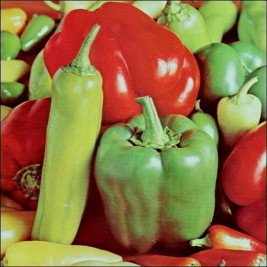
\includegraphics[width=0.25\textwidth]{figures/peppers.jpg}
\end{figure}

Decrease numerical precision to speed up the computation:

\begin{Verbatim}
    --> import "convolution.lisp"
    OK
    --> let ((fr 10)) (img:write "peppers-blurry.jpg" (convolve-rgb
    ...     (img:read "peppers.jpg")
    ...     (* (/ 9) '((1 1 1) (1 1 1) (1 1 1)))))
    peppers-blurry.jpg
\end{Verbatim}

\begin{figure}[h]
    \caption{peppers-blurry.jpg}
    \centering
    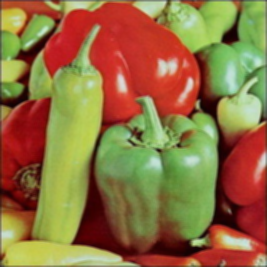
\includegraphics[width=0.25\textwidth]{figures/peppers-blurry.jpg}
\end{figure}

Another interesting operation to check is the Gaussian blur:

\begin{Verbatim}
    --> import "convolution.lisp"
    OK
    --> let ((fr 10)) (img:write "peppers-gauss.jpg" (convolve-rgb
    ...     (img:read "peppers.jpg")
    ...     (* (/ 16) '((1 2 1) (2 4 2) (1 2 1)))))
    peppers-gauss.jpg
\end{Verbatim}

\begin{figure}[h]
    \caption{peppers-gauss.jpg}
    \centering
    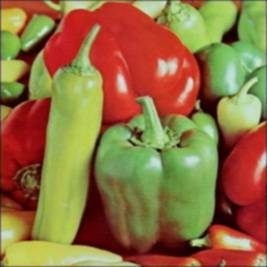
\includegraphics[width=0.25\textwidth]{figures/peppers-gauss.jpg}
\end{figure}

Finally, the edge detection kernel:

\begin{Verbatim}
    --> import "convolution.lisp"
    OK
    --> let ((fr 10)) (img:write "peppers-edge.jpg" (convolve-rgb
    ...     (img:read "peppers.jpg")
    ...     '((-1 -1 -1) (-1 8 -1) (-1 -1 -1))))
    peppers-edge.jpg
\end{Verbatim}

\begin{figure}[h]
    \caption{peppers-edge.jpg}
    \centering
    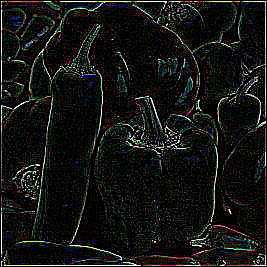
\includegraphics[width=0.25\textwidth]{figures/peppers-edge.jpg}
\end{figure}

\section{Searching and partitioning}

\section{Sorting and permutations}

\section{Pattern matching}

\section{Sets}

\section{Hashmaps}

\section{Using glyphs}
